\chapter{Network Design}

\section{Topology}

The topology used for this lab assignment takes the form of a three router set-
up, simulating the infrastructure a typical Internet Service Provider (ISP)
might have. Using three routers as opposed to a one allows the ISP to make use
of additional technologies such as dynamic internal routing and iBGP in order
to create a fault-tolerant network. Using multiple devices results in increased
uptime as traffic can be routed via an alternate path should any outage occur
on any single device.

\begin{figure}[!ht]
    \caption{High-level Topology}
    \centering
    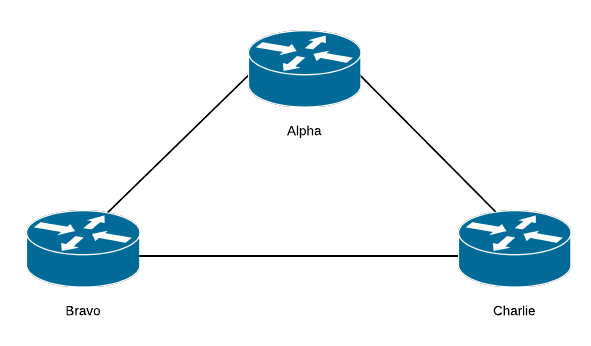
\includegraphics[width=0.8\textwidth]{images/networkTopology.png}
\end{figure}

\section{Address Allocation}
\subsection{IPv4}
For this lab exercise we represent the ISP BT and are assigned the IP block
\texttt{12.0.0.0/8} for our network. This address space provides us with 16.7
million addresses to allocate, of which we require only a small fraction.
However taking into account the issues that arose from the original allocation
of excessive IPv4 network blocks to ISPs and Educational Institutions, we
decided it was best to be conservative in our allocations. With this in mind we
invented three classifications of network address, each defining the minium
subnet size deemed necessary for its purpose. These are outlined in
Figure~\ref{figure:network-alloc-1}.

\begin{figure}[!ht]
    \caption{Classifications of Network Allocations}
    \label{figure:network-alloc-1}
    \centering
    \begin{tabular}{|c|c|p{5.5cm}|}

        \hline
        \textbf{Address Type} & \textbf{Subnet Mask} & \textbf{Justification} \\

        \hline
        Customer Segment & \texttt{/24} & These are allocated to
        downstream customers, who are given enough address space for 254
        devices. In our network, laptops are used on these segments to test
        connectivity to customers. The size of this subnet also allows for easy
        identification of subnets to their location in the topology.\\

        \hline
        Point-to-point Links & \texttt{/30} & This is used for links that
        connect two routers, because for these links only two IP Addresses are
        required and a \texttt{/30} subnet mask is the smallest mask that will
        provide this.\\

        \hline
        Loopback Address & \texttt{/32} & Addresses used for the loopback
        interfaces on the routers, there is only a requirement for a single
        address and a \texttt{/32} mask produces this.\\

        \hline
    \end{tabular}
\end{figure}

In addition to the allocation of subnets based on size, the ISP also uses the
addresses encompassed in the block as an identifier for it's location in the
network. Using the value of a particular octet in a network address was a schema
that was created in advance of the network build-out and allowed for easy
identification of issues in IP or interior routing configurations. These schemas
are outlined in Figure~\ref{figure:network-alloc-2}.

\begin{figure}[!ht]
    \caption{Network Allocations}
    \label{figure:network-alloc-2}
    \centering
    \begin{tabular}{|c|p{8cm}|}
        \hline
        \textbf{Address Allocation} & \textbf{Identifying Feature} \\

        \hline
        \texttt{12.0.\#.0/24} & The hash in this address dictates the router that
        this address space is connected to, with 1 corresponding to Alpha etc.
        This would scale for up to 253 subnets in the Service Provider.\\

        \hline
        \texttt{12.\#.0.0/30} (10+) & The hash in these networks dictate the assigned
        number of the group we connect to on these links. This enables us to
        quickly identify the group involved with any connectivity issues in
        BGP.\\

        \hline
        \texttt{12.\#.\#.\#} & This schema was used for loopback addresses on the
        routers, the hash is the same value in all three octets of the address
        and dictates the router that this loopback is assigned to. For example,
        \texttt{12.3.3.3/32} is the loopback address of Charlie.\\
        \hline
    \end{tabular}
\end{figure}
\clearpage

\subsection{IPv6}